\section{Current Work: Video as a Scalable Foundation for Predictive Multimodal Learning}

\begin{frame}{\Large Why Video for Predictive Multimodal Learning?}
  \centering
  \vspace{0.20cm}
  {\fontsize{10}{12}\selectfont
  \[
  \begin{aligned}
  \textbf{Past work:}\quad
  & o_t
    \xrightarrow{\;\text{Model}_{\text{\tiny perceive, reason, act}}\;}
    y_t
  \\[0.85em]
  \textbf{Agent rollout:}\quad
  & o_t \xrightarrow{\;a_t\;} o_{t+1},
    \qquad
    (o_1, a_1, o_2, a_2, \ldots, o_T)
  \\[0.85em]
  \textbf{Video rollout:}\quad
  & o_t \xrightarrow{\;u_t\;} o_{t+1},
    \qquad
    (o_1, u_1, o_2, u_2, \ldots, o_T)
  \\[0.85em]
  \textbf{Prediction:}\quad
  & \text{estimate future observations under transition drivers}
  \end{aligned}
  \]
  }

  \vspace{-0.06cm}
  {\fontsize{7.7}{9}\selectfont
  \(o_t\): multimodal observation \([\,\text{frames} \mid \text{language} \mid \text{audio} \mid \cdots\,]\) \\
  \(a_t\): explicit agent action
  \quad
  \(u_t\): unobserved video dynamics}

  \vspace{0.20cm}
  \begin{tikzpicture}
    \node[
      rounded corners=5pt,
      draw=AgentBlueDark!50,
      fill=AgentBlue!18,
      thick,
      minimum width=10.75cm,
      minimum height=0.64cm,
      align=center,
      inner sep=4pt
    ] {\scriptsize Video is a scalable entry point for learning how multimodal states evolve over time.};
  \end{tikzpicture}
\end{frame}

\molochset{progressbar=foot}

\begin{frame}{\Large Video Data Foundations for Predictive Multimodal Learning}
  \centering
  \vspace{0.18cm}
  {\fontsize{10}{11}\selectfont\textbf{Video curation to build better predictive models.}}

  \vspace{0.72cm}
  \begin{tikzpicture}[
    stage/.style={
      rounded corners=5pt,
      draw=AgentBlueDark!55,
      fill=AgentGray,
      very thick,
      minimum width=2.25cm,
      minimum height=1.02cm,
      align=center,
      inner sep=4pt
    },
    modelbox/.style={
      rounded corners=5pt,
      draw=AgentOrangeDark!70,
      fill=AgentOrange!45,
      very thick,
      minimum width=2.45cm,
      minimum height=0.76cm,
      align=center,
      inner sep=4pt
    },
    arrow/.style={-Latex,thick,draw=AgentBlueDark!78}
  ]
    \node[stage] (raw) at (-5.25,0) {\small\textbf{Raw Videos}\\[-0.20em]\scriptsize web-scale source};
    \node[stage] (seg) at (-2.35,0) {\small\textbf{Segmentation}\\[-0.20em]\scriptsize semantic clips};
    \node[stage] (filter) at (0.55,0) {\small\textbf{Filtering}\\[-0.20em]\scriptsize quality control};
    \node[stage] (anno) at (3.45,0) {\small\textbf{Annotation}\\[-0.20em]\scriptsize captions / metadata};

    \node[modelbox] (gen) at (6.35,0.70) {\small\textbf{Video Gen}\\[-0.18em]\tiny generative prediction};
    \node[modelbox] (jepa) at (6.35,-0.70) {\small\textbf{V-JEPA}\\[-0.18em]\tiny self-supervised prediction};

    \draw[arrow] (raw.east) -- (seg.west);
    \draw[arrow] (seg.east) -- (filter.west);
    \draw[arrow] (filter.east) -- (anno.west);
    \draw[arrow] (anno.east) -- (gen.west);
    \draw[arrow] (anno.east) -- (jepa.west);
  \end{tikzpicture}

  \vspace{0.50cm}
  {\fontsize{9}{10}\selectfont
  \textbf{Evaluation:} controlled curation variants \(\rightarrow\) matched-budget pretraining \(\rightarrow\) predictive capability probes.}

  \vfill
  \begin{flushright}
    {\fontsize{5.5}{5}\selectfont \textcolor{darkgray}{[Ongoing Project]~~\textit{Which Video Curation Practices Matter for Predictive Model Pretraining?}}}
  \end{flushright}
\end{frame}

\molochset{progressbar=foot}

\begin{frame}{\Large Future Vision: Three Generations of Multimodal Agents}
  \centering
  \vspace{0.04cm}
  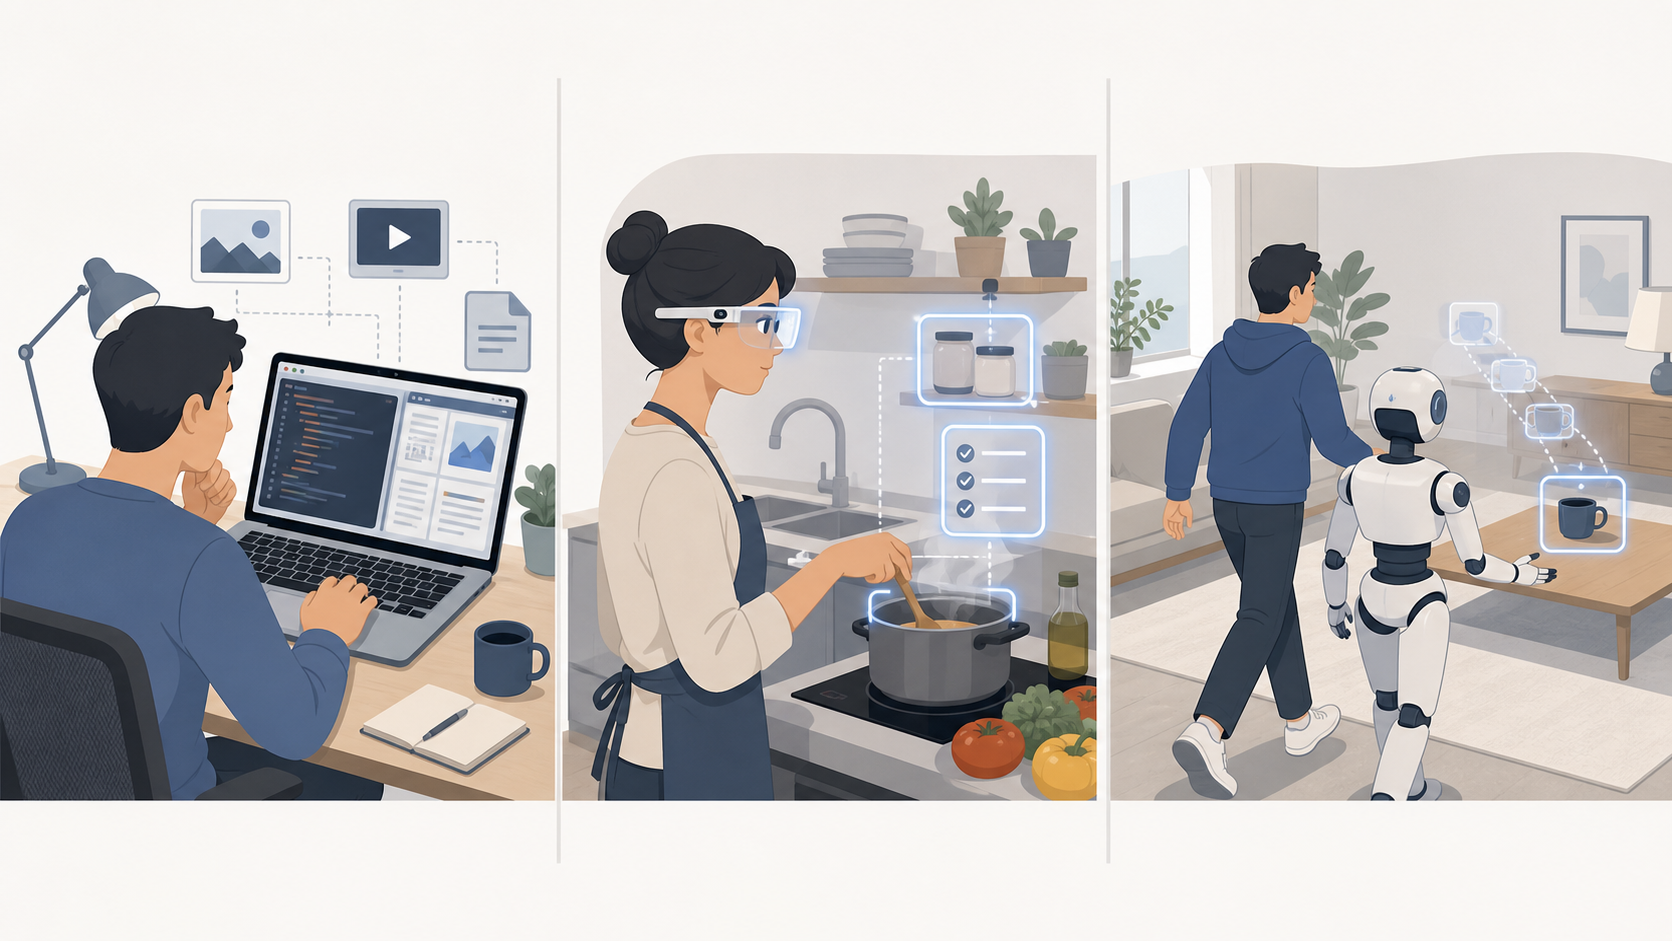
\includegraphics[
    width=0.75\linewidth,
    trim={0 70 0 55},
    clip
  ]{figures/current_future/real_world_multimodal_agents.png}

  \vspace{-0.50cm}
  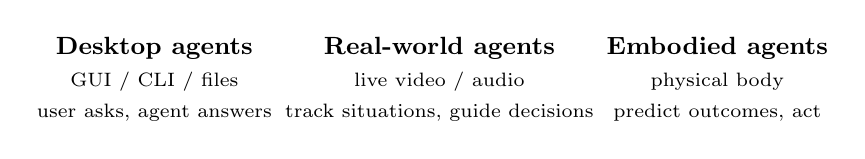
\begin{tikzpicture}
    \node[align=center] at (-4.00,0) {
      {\small\textbf{Desktop agents}}\\[-0.05em]
      {\fontsize{7.0}{7}\selectfont GUI / CLI / files}\\[-0.05em]
      {\fontsize{7.0}{7}\selectfont user asks, agent answers}
    };
    \node[align=center] at (-0.38,0.) {
      {\small\textbf{Real-world agents}}\\[-0.05em]
      {\fontsize{7.0}{7}\selectfont live video / audio}\\[-0.05em]
      {\fontsize{7.0}{7}\selectfont track situations, guide decisions}
    };
    \node[align=center] at (3.15,0.) {
      {\small\textbf{Embodied agents}}\\[-0.05em]
      {\fontsize{7.0}{7}\selectfont physical body}\\[-0.05em]
      {\fontsize{7.0}{7}\selectfont predict outcomes, act}
    };
  \end{tikzpicture}

  \vspace{0.24cm}
  {\fontsize{8.0}{10}\selectfont
  Toward agents that
  \textcolor{PerceiveColor}{\textbf{perceive}} live environments,
  \textcolor{ReasonColor}{\textbf{reason}} over evolving situations,
  \textcolor{ActColor}{\textbf{act}} through tools or bodies,
  and \textcolor{PredictColor}{\textbf{predict}} what comes next.}
\end{frame}

\molochset{progressbar=foot}
